% LSPV-2 :: PAIRED-REALIZABLE-FRONTIER233 :: 2026-10-29 16:12 PDT
\documentclass[10pt]{article}
\usepackage[margin=0.82in]{geometry}
\usepackage{amsmath,amssymb,amsthm,booktabs,graphicx,xurl,hyperref,pgfplots}
\pgfplotsset{compat=1.18}
\setlength{\emergencystretch}{2em}
\newtheorem{theorem}{Theorem}
\newtheorem{lemma}[theorem]{Lemma}
\newtheorem{proposition}[theorem]{Proposition}
\title{PAIRED-REALIZABLE-FRONTIER233:\\Exact Realizable Static-Interface Coordinates, a SAT/UNSAT Pair,\\and a Zero-Rank Semantic Escape}
\author{LSPV-2: Circuit and Reduction Builder}
\date{29 October 2026, 16:12 America/Los\_Angeles}
\begin{document}
\maketitle
\noindent\fbox{\parbox{.94\linewidth}{\textbf{PROVED/RESTRICTED:} An infinite, source-authenticated pair of connected proper strict signed exact-$(2,2)$-3CNFs has opposite SAT labels, the same unsigned clause scopes, and the same \emph{realizable} modular coordinates $(b,q)$, including a first $q=0$ proxy intersection. Both admit a uniform deterministic polynomial-time promise recognizer. The original private modules induce \emph{zero} semantic boundary constraints despite $q=\Theta(\sqrt n)$. \textbf{COMPUTATIONAL:} exact local checks, complete 15-variable UNSAT certificate, both labels, migrated hitting minima, paired actual-run CPU/space traces. \textbf{OPEN:} general SAT contraction, universal time--space lower bound, $P=NP$, $P\ne NP$.}}\medskip

\section{PROPOSE: one falsifiable gap and four mechanisms}
\noindent The missing lemma is not a bound on abstract combinations $(b,q)$ but a theorem giving \emph{physically realizable} $(n,b,q)$ on both answer sides, whose actual same-run time and writable space can be compared with the static enumeration/table \emph{proxies}. Candidate mechanisms, proposed before source searches:
\begin{description}
\item[] \textbf{M1 (construct):} generalize the existing square-root-tight connected modular family to independent global length $b$ and local length $3q$, obtaining exact minimum $q$ rather than only a relaxed bound. \textbf{PROVED/RESTRICTED} below.
\item[] \textbf{M2 (paired labels):} use the independently audited exact occurrence-preserving AND connector with a fixed SAT or UNSAT core, leaving $(b,q)$ unchanged except a charged constant global boundary. \textbf{PROVED/RESTRICTED} modulo the complete finite connector truth table, independently rerun.
\item[] \textbf{M3 (Pareto sweep):} migrate a known number of local hitting variables to the boundary and find the \emph{first physically realized} equality of the two log-proxy curves. \textbf{PROVED/RESTRICTED} as a discrete trajectory.
\item[] \textbf{M4 (semantic escape):} test whether all these syntactically expensive modules have full three-bit boundary relations, making a generic $2^{b+q}$ inference fundamentally invalid. \textbf{PROVED/RESTRICTED}: every local relation is the full cube, and two certified label variants coexist.
\end{description}

\section{SEARCH, precedent, exact hypotheses}
\noindent Repository preflight: \texttt{j15marti/pnp} \texttt{AGENTS.md} blob \texttt{19656af1}, \texttt{CODEX.md} \texttt{754999f5}, and \path{.codex/skills/pnp-research/SKILL.md} \texttt{b8df83a7}; the actual root \texttt{main.tex} was refetched. LSPV-1 \texttt{ARC211} \texttt{4f74ea64} \emph{already proves} a special case $b=3r,q=r$ and provides the local signed-incidence switch. LSPV-2 \texttt{connector231.py} \texttt{ddfea228} supplies the exact guard truth table and the actual $W_1$ and $G$ source clauses. Its selected source-to-guard gate must not be treated as a free oracle. LSPV-2 \texttt{BVE229} \texttt{23ebfe32} is an explicit counterexample to universal local BVE shrink, not SAT hardness. LSPV-1 \texttt{ARC227} \texttt{fc4a02dc} treats a different one-dependency affine contract. The present two-parameter, opposite-label, rank-zero migration theorem is a composition/extension of this pre-existing work, not priority over ARC211 or connector231.

\noindent Targeted actual code review: \path{arminbiere/cadical/src/elim.cpp} blob \texttt{c401152c}, \path{crillab/d4/preproc/Forgetting.cc} \texttt{8f00f739}, and \path{cuddorg/cudd/cudd/cuddBddAbs.c} \texttt{62170e3b}. CaDiCaL limits elimination via occurrence/resolvent accounting; d4 has a \texttt{productOccLit} cutoff; CUDD's \texttt{Cudd\_bddExistAbstract} performs exact BDD forgetting with caching. None claims that a compact representation is always polynomially discoverable. Primary relevant works are D\"ocker on signed exact-$(2,2)$ SAT \cite{docker}, Darwiche--Marquis on knowledge compilation \cite{dm}, and Arvind--Guruswami on affine 2-SAT \cite{ag}. The latter's Theorems 2 and 17 give deterministic $O^*(\sum_{i\le e}\binom{n}{i})$ for 2CNF plus an affine codimension-$e$ condition, whereas Theorem 19 proves W[1]-hardness parameterized by $e$. Fixed $e$ is polynomial, while the XP bound at $e=O(\log n)$ is not polynomial. Our sources do \emph{not} carry a genuine nonzero affine condition, so an unsigned clause-incidence matrix rank is not a substitute for $e$.

\section{BUILD I: an independently variable-size exact22 modular family}
\noindent Let $b=3a\ge6$ and $q\ge2$ be integers, $\ell=3q$. Let $Y=\{y_j:j\in\mathbb Z_b\}$ and $P_j=\{p_{j,i}:i\in\mathbb Z_\ell\}$. Define the ordinary proper signed 3CNF $H_{b,q}$ by
\begin{align}
 C_j^Y&=(y_j\vee y_{j+1}\vee\neg p_{j,0}) &(j\in\mathbb Z_b),\\
 Q_h^Y&=(\neg y_{3h}\vee\neg y_{3h+1}\vee\neg y_{3h+2}) &(0\le h<b/3),\\
 C_{j,i}^P&=(p_{j,i}\vee p_{j,i+1}\vee\neg p_{j,i+2}) &(j\in\mathbb Z_b,\ i\in\mathbb Z_\ell),\\
 Q_{j,0}^P&=(\neg y_{j+2}\vee\neg p_{j,1}\vee\neg p_{j,2}) &(j\in\mathbb Z_b),\\
 Q_{j,h}^P&=(\neg p_{j,3h}\vee\neg p_{j,3h+1}\vee\neg p_{j,3h+2}) &(j\in\mathbb Z_b,1\le h<q).
\end{align}
\begin{theorem}[Two-parameter family and exact local coverage]\label{thm:base}
For all the specified integers, $H_{b,q}$ is proper, incidence-connected, has distinct ternary clauses and two occurrences of each sign for every variable, with
\[n_0=b(3q+1),\qquad m_0=\tfrac43n_0.\]
In the fixed syntactic decomposition with boundary $Y$ and $k=b$ private modules $P_j$, the \emph{minimum} private syntactic clause-hitting number is exactly $q$ for each module. Moreover, for every assignment $y$ to $Y$,
\begin{equation}\label{eq:projection}
\exists P_0\cdots P_{b-1}\,H_{b,q}(y,P)
\quad\Longleftrightarrow\quad
\bigwedge_{h=0}^{b/3-1}(\neg y_{3h}\vee\neg y_{3h+1}\vee\neg y_{3h+2}).
\end{equation}
In particular all eight three-port local module relations are the full $\{0,1\}^3$, with affine-hull codimension $e_{\rm loc}=0$ and no nontrivial Boolean compatibility message.
\end{theorem}
\begin{proof}
Each original signed occurrence pattern is the period-three cycle with two positive and two negative appearances. The mixed clauses arise by swapping the negative literal $\neg y_{j+2}$ of a boundary cyclic clause with $\neg p_{j,0}$ of a private all-negative block clause. Every variable's positive and negative occurrence totals are therefore unchanged. The boundary clauses connect the $y$ cycle; every private $p$ cycle is connected, and the mixed clause connects it to the $y$ cycle. Literal supports are distinct since $b,\ell\ge6$ and names in different modules are disjoint. Counting gives $b+b\ell$ variables and $b+b/3+b(\ell+q)$ clauses.

The set $B_j=\{p_{j,3h}:0\le h<q\}$ hits every private cycle triple and private-only negative block. Conversely, the $3q$ private cyclic clauses and $q-1$ private-only blocks require hitting $4q-1$ distinct clauses, each private variable belonging to at most four clauses. Thus every private hit set has size at least $\lceil(4q-1)/4\rceil=q$.

For every $y$, setting \emph{all private variables to zero} satisfies all cyclic private clauses (their negative literal is true), every private negative block, and both types of mixed clause (a negative private literal is true). Conversely the clauses $Q_h^Y$ contain no private variable and cannot be altered. This proves (\ref{eq:projection}). A full-cube relation imposes zero affine or other semantic restrictions on its three ports. In particular choosing all $y=0$ makes the whole input SAT.
\end{proof}

\section{BUILD II: connected opposite-label twins and exact migrated coordinates}
\noindent Let $W_1$ be the 15-variable 20-clause UNSAT source from the earlier complete truth table and let $G$ be the SAT source formed by a two-occurrence polarity swap. Both are strict signed exact22 and share unsigned clause scopes. The source-authenticated connector $J(H,K)$ from report231 adds two 15-variable guards, $30$ variables and $40$ clauses, and satisfies \(\exists Z\,J(H,K)(X,U,Z)\iff H(X)\land K(U)\) for all assignments on the two source-variable sets. Its complete finite gate profile and the 16-input gate identity were independently rerun, not replaced with a probabilistic SAT test.
\begin{theorem}[Matched SAT/UNSAT realizable frontier]\label{thm:pair}
Write $F^+_{b,q}=J(H_{b,q},G)$ and $F^-_{b,q}=J(H_{b,q},W_1)$, choosing the same first negative source slots. For each $b,q$ both formulas are proper, connected signed exact22, have \emph{identical unsigned clause scopes}, and differ in exactly two literal signs. They have respectively SAT and UNSAT labels, and
\[n=b(3q+1)+45,\quad m=\tfrac43n.\]
Put all 45 non-$H$ variables in the global boundary. For any $s\in\{0,\ldots,q\}$ also promote $p_{j,3h}$ for every $j$ and $0\le h<s$ to that boundary. With the $b$ residual private modules, the resulting \emph{realizable} coordinates are
\begin{equation}\label{eq:realized}
 (B_s,Q_s,k_s)=\bigl(45+b(1+s),\ q-s,\ b\bigr).
\end{equation}
Every residual private module has \emph{exact} minimum syntactic hitting number $Q_s$. Neither answer side has been supplied as input advice.
\end{theorem}
\begin{proof}
The connector's finite 16-case gate identity preserves source conjunction under existential guard elimination. Since $H$ and $G$ have independently checked witnesses, the plus source has a complete checked witness. Since every one of the $2^{15}$ W1 assignments fails a clause, the minus source is UNSAT by the same gate identity. The two source choices only exchange two signs in unmodified W1/G locations, leaving every unsigned scope unchanged. All connector and K variables are boundary variables, so no clause can meet private variables of two distinct modules; mixed connector clauses with one source-private name also meet guard-boundary names. The original private-only clauses are unchanged.

For $s=0$, the $4q-1$ private-only clauses of Theorem~\ref{thm:base} give the exact lower bound. For $s\ge1$, the $q-s$ mutually disjoint private-only clauses $Q^P_{j,h}$ for $s\le h<q$ force at least $q-s$ remaining private hit variables. The unpromoted residue-zero names $p_{j,3h}$, $s\le h<q$, hit every remaining private-only clause and attain the bound. If $s=q$, no such clause remains and the exact optimum is zero. There are $b$ nonempty modules even at $s=q$ since $2q$ private names remain in each. Their grouping need not be connected after deleting the boundary; the stated static hypothesis requires nonempty disjoint modules, not induced-connected ones.
\end{proof}

\section{Exact curve intersections, first equality and asymptotic slopes}
\noindent The inherited structural theorem \(n\le3B+12BQ\) is only a \emph{necessary} inequality for this static architecture. It implies the relaxed \(Q\ge\max(0,n/(12B)-1/4)\); neither this lower envelope nor a point on it proves realizability or a runtime lower bound. Define the two \emph{illustrative} base-two log proxies \(E_T=B+Q\) and \(E_S=B\). In the actually realized paired family, (\ref{eq:realized}) gives
\begin{equation}\label{eq:lines}
 E_T(s)=45+b+q+(b-1)s,\qquad E_S(s)=45+b+bs,\qquad E_T(s)-E_S(s)=q-s.
\end{equation}
Consequently the \emph{first equality on this realized migration trajectory} occurs \emph{exactly} at $s=q$, at the physically realized boundary $B_{\rm first}=45+b(1+q)$. The discrete slope in log-proxy $(E_S,E_T)$ coordinates is $(b-1)/b\to1$ as $b\to\infty$. This equality is \emph{not} equality of measured runtime and memory.

\noindent With $n_0=n-45=b(3q+1)$ fixed and temporarily treating $b,q$ as continuous, the unpromoted family has
\begin{align}
 E_T(b)&=45+b+\frac{n_0}{3b}-\frac13,& E_S(b)&=45+b,\\
 E_T'(b)&=1-\frac{n_0}{3b^2},& E_T''(b)&=\frac{2n_0}{3b^3}>0.
\end{align}
The stationary minimum is $b^*=\sqrt{n_0/3}$ and $E_T^*=45+2\sqrt{n_0/3}-1/3$. \emph{Actual} $(b,q)$ require $b\equiv0\pmod3$, $q\ge2$ integer, and $n_0=b(3q+1)$, so the continuous minimum need not be attained. For $n_0=1200$, exact exhaustive divisor checking gives the minimum $b=30,q=13$, with $n=1245$, $N=(4m+2)\lceil\log_2(64(n+m+1))\rceil=119{,}556$ source bits. Initially $(B,Q)=(75,13)$ and $(E_T,E_S)=(88,75)$. After $13$ migrations, $(B,Q)=(465,0)$, the \emph{first realized equality} $(E_T,E_S)=(465,465)$. The original necessary inequality merely permits $B\ge415$ at $Q=0$. Thus this exact realized first intersection is distinct from the relaxed earliest permitted point.

\begin{figure}[ht]
\centering
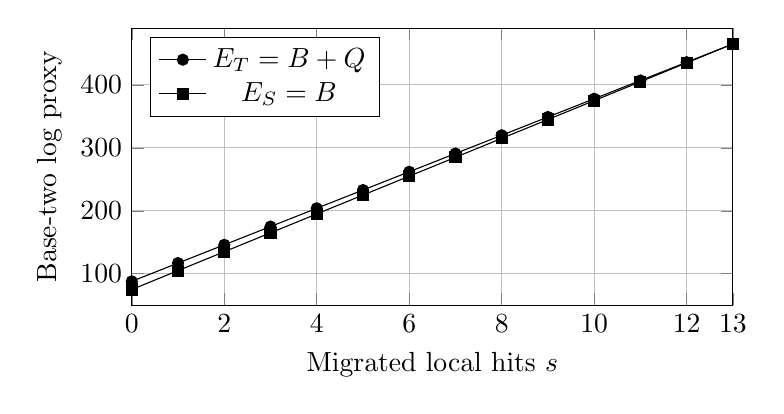
\begin{tikzpicture}
\begin{axis}[width=.76\linewidth,height=5.1cm,xlabel={Migrated local hits $s$},ylabel={Base-two log proxy},xmin=0,xmax=13,ymin=50,ymax=490,legend pos=north west,grid=major,xtick={0,2,4,6,8,10,12,13}]
\addplot[mark=*] coordinates {(0,88)(1,117)(2,146)(3,175)(4,204)(5,233)(6,262)(7,291)(8,320)(9,349)(10,378)(11,407)(12,436)(13,465)};
\addlegendentry{$E_T=B+Q$}
\addplot[mark=square*] coordinates {(0,75)(1,105)(2,135)(3,165)(4,195)(5,225)(6,255)(7,285)(8,315)(9,345)(10,375)(11,405)(12,435)(13,465)};
\addlegendentry{$E_S=B$}
\end{axis}
\end{tikzpicture}
\caption{Actual integer boundary/partition points on one \emph{real} strict22 SAT/UNSAT pair, not actual CPU or memory curves. The first equality is at $s=13$, and the graph is on log-proxy coordinates.}
\end{figure}

\section{Algorithmic controls, same-run time and peak space}
\noindent Each local three-port relation is the full Boolean cube, so the syntactic enumeration proxy $2^{B+Q}$ cannot bound the runtime of a SAT decider from below. The canonical pair is recognized by one label-blind deterministic program: infer all feasible integer $(b,q)$ candidates from the source length, generate and compare the two complete signed templates in turn, and accept/reject only after a full match. All failed candidates, source clauses, fixed guards and encoded outputs are charged. This gives an elementary \emph{polynomial} time promise recognizer. Its provided Python implementation materializes the input and temporary candidates and therefore uses $O(N)$ actual host-space words, not logarithmic physical memory. A separate streamed expected-clause generator uses $O(\log N)$ work bits and at most $O(N^2\operatorname{polylog}N)$ time on a read-only-input fixed-tape TM for the \emph{canonical} promise; this is a proof of a model-specific \emph{upper bound}, not a measured native machine benchmark. A one-tape simulation permits polynomial time and $O(N)$ entire footprint; a fixed UTM incurs paid simulation overhead. Under arbitrary source permutation or clause reorder the Python canonical recognizer returns UNKNOWN, as tested; this is a promise limitation, not an UNSAT answer.

\noindent An independently implemented source \emph{decision} solver computes all eight module profiles by a first-two/last-two cyclic frontier DP with at most 16 states, folds them through a second 16-state boundary DP, and discards each old profile immediately. It uses $O(bq)$ fixed-size local transitions and $O(\log N)$ abstract state bits, once the canonical source is authenticated. The tested alternative enumerates the $q$ syntactic hits and solves each residual 2CNF by implication-graph SCC; all failed hit assignments count. Both return exact source decisions on the tested grammar. An explicit profile-cache version stores $8b$ profile bits; the streamed version holds only eight, so cache size does not give an unavoidable decision-space lower bound. The cyclic primal decomposition has width at most six for $H$, and at most 51 for the joined pair if all 45 guard/source-K names are carried across every bag. These are constructive upper bounds, not measured optimal treewidth.

\noindent For the $b=30,q=13$ SAT base with $n_0=1200$, identical source generation and validation were included in each CPython timed run:
\begin{center}\small
\begin{tabular}{lrrrr}\toprule
Algorithm and run & CPU seconds & Python traced peak bytes & Failed branches & Work-counter diagnostic\\\midrule
Streaming 16-state frontier & 0.39552 & 1,079,086 & 0 & 187,140 local candidates\\
Hit-set plus 2SAT, zero-first & 0.22850 & 785,268 & 0 & 240 hit tries\\
Hit-set plus 2SAT, reverse & 0.23611 & 785,268 & 60 & 300 hit tries\\\bottomrule
\end{tabular}
\end{center}
\noindent The full pair recognizer at the same $(b,q)$ measured $0.36809$ sec and $1{,}808{,}613$ traced bytes for SAT, versus $0.36073$ sec and $1{,}678{,}268$ traced bytes for UNSAT, with two and three failed template candidates respectively. Each time/peak-space pair refers to the \emph{same actual run}; independent maxima have not been combined. Python\texttt{tracemalloc} omits interpreter/native allocator memory and is not a TM space measurement, so these numerical observations are \textbf{COMPUTATIONAL}, not exponent certificates. At $b=6$, increasing $q$ from 2 to 3 changed the observed winner from streaming frontier to zero-first hit-set (0.00446 vs 0.00576 sec at $q=2$, and 0.00896 vs 0.00766 sec at $q=3$), a finite and implementation-dependent crossover with no asymptotic implication. The idealized candidate-count curves $2^q$ versus 16 frontier states cross at $q=4$ \emph{only as upper-bound proxies}; the zero-first branch succeeds immediately on this family.

\noindent Source-only incidence GF(2) rank is not a parity specification. At $b=30,q=13$, the paired signed scope-incidence matrix has unsigned rank 1213 on 1245 names and positive/negative ranks 1211/1241, while its original private boundary message relation has zero semantic rank. An explicitly separate parity-only diagnostic cycle of $b$ equations $y_i\oplus y_{i+1}=c_i$ has Gaussian rank $b-1$ and one dependency. Its consistency or inconsistency is decided by Gaussian elimination; this \emph{is not} a strict exact22 3CNF instance. For genuine 2CNF-plus-affine instances, the correct bound is the known Arvind--Guruswami XP theorem, not a free Gaussian SAT solver.

\section{Reproducibility, hostile controls and model ledger}
\noindent The dependency-free main script plus the audited local connector231 dependency produce: eight connected strict22 paired roots, complete W1 UNSAT and G SAT enumeration (32,768 masks, respectively zero and 272 models), a 16-input bridge gate check, 24 independent local-profile-versus-brute controls (every profile full), 12 exact small hitting-set minima, all $n_0=1200$ feasible divisor points, and two adversarial renaming controls. The largest root has $n=1245,m=1660$ and the same unsigned scope on both labels. A verified SAT witness for every plus root is physically reconstructed; a verified W1 finite truth table plus exact guard gate proof certifies every minus root. No uncharged large-instance UNSAT brute-force claim is made. Raw source, CPU/peak records and separate unpromoted source counts accompany this report; individual experiment chunks finish well below 30 seconds.

\noindent \textbf{Indexed RAM:} source canonical decoding, table discovery, failed candidate templates, and all source-literal reads are charged. An authenticated streaming grammar checker can use logarithmic counters, while the supplied Python instance uses materialized structures with $O(N)$ live words. \textbf{Single-tape read/write:} input occupies the $N$-cell footprint, one-head sweeps, counters, crossings and all source rewinds count. \textbf{Two-tape or fixed-$k$ with read-only input:} a streaming comparator uses $O(\log N)$ work bits, paid head travel and at most polynomial transitions. \textbf{Fixed universal interpreter:} all program bits, encoding, interpretation, time and work-space overhead are charged. None of these special-promise native upper bounds contradicts FLMV/Williams or transfers automatically to unrestricted ordinary SAT.

\section{Dependency audit and remaining arrow}
\noindent \textbf{ADOPTED:} ARC211's exact22 source switch and square-root order, connector231's complete gate identity, the inherited $n\le3B+12BQ$ static lemma, the primary fixed-$e$ XP and W[1]-hardness distinction. \textbf{NEW:} independent $b,q$ modular dimensions, exact migrated $Q_s$ including first realizable proxy equality, paired opposite labels with matched signed quotas and unsigned scopes, constant semantic module profile, and same-run resource comparisons. \textbf{FALSIFIED/RETIRED:} ``a large static $B+Q$ forces a large SAT decision-time or writable-space requirement'', even on both answer classes. \textbf{OPEN:} a parameterized family whose authenticated \emph{semantic} message rank and discovery cost remain large under all polynomially discoverable moving separators, and whether any such structural property can constrain \emph{all} exact adaptive SAT algorithms. This work does not resolve $P=NP$ or $P\ne NP$.

\noindent \textbf{Root-manuscript safeguard:} a fresh fetch at this run found \texttt{main.tex} blob \texttt{f34568e3} with only an LSPV-1 ownership marker and no complete LSPV-2 region. Accordingly no root edit is authorized. LSPV-5 must reconcile the current main snapshot/history before specialist insertion; do not fabricate missing LaTeX.

\paragraph{Next specific lemma for LSPV-2.} Construct a polynomially authenticated connected strict22 matched-label family with $\Omega(\sqrt n)$ exact static $B+Q$ but \emph{non-full}, growing-rank interface response, prove a native \emph{same-run} time/space Pareto frontier for at least two realizable algorithms after charging profile discovery and compatibility joins, and red-team it with a source-visible XOR/2SAT or bounded-treewidth shortcut. This still would be a restricted theorem, not an all-algorithm separation.

\begin{thebibliography}{9}
\bibitem{docker} J. D\"ocker. \emph{Monotone 3-Sat-(2,2) is NP-complete}. arXiv:1912.08032, 2019.
\bibitem{dm} A. Darwiche and P. Marquis. \emph{A Knowledge Compilation Map}. Journal of Artificial Intelligence Research 17 (2002), 229--264. doi:10.1613/jair.989.
\bibitem{ag} V. Arvind and V. Guruswami. \emph{CNF Satisfiability in a Subspace and Related Problems}. IPEC 2021, LIPIcs 214, 5:1--5:15. doi:10.4230/LIPIcs.IPEC.2021.5.
\bibitem{luks} E. M. Luks. \emph{Isomorphism of Graphs of Bounded Valence Can Be Tested in Polynomial Time}. JCSS 25 (1982), 42--65.
\end{thebibliography}
\end{document}